\documentclass[a4paper,12pt]{article}
\usepackage[utf8]{inputenc}
\usepackage[ngerman]{babel}
\usepackage[a4paper, left=2.5cm, right=2.5cm]{geometry}
\usepackage{graphicx}
\usepackage{subcaption}
\usepackage{fancyhdr}
\usepackage{pdfpages}
\usepackage{longtable}
\usepackage{multirow}
\usepackage{pgfplots}
\usepackage{pgfplotstable}
\usepackage{float}
\pagestyle{fancy}
\lhead{Messtechnik Labor}
\chead{}
\rhead{Gruppe 2}

\begin{document}
	
\includepdf{LU6_Protokoll_titlepage.pdf}
	
	\noindent
	\textbf{\Large Rechtliches} \\ \\
	Ich bestätige hiermit, dass alle hier verwendeten Messergebnisse und Interpretationen von uns selbst erstellt wurden. Es wurden keine anderen Quellen als die hier schriftlich angegeben verwendet.
	\setcounter{page}{2}
	
	\newpage
	%Inhaltsverzeichnis
	\tableofcontents
	
	\newpage
	\section{Einleitung}
	Die sechste Laborübung ist in zwei Teile gegliedert.\\ \newline
	Der erste Teil beschäftigt sich mit der Positionsmessung durch einen optischen Näherungssensor. Hier werden die Grundlagen der optischen Abstandsmessung erforscht, wie zum Beispiel das Ermitteln der Kennlinie, die Charakterisierung in Bezug auf Rauschen, Sensitivität, Auflösung und Bandbreite eines optischen Näherungssensors.\\ \newline
	Der zweite Teil geht näher auf die Eigenschaften eines phasenselektiven	Synchrongleichrichters und eines phasenunabhängigen Synchrondemodulators ein. Anhand der Erkenntnisse aus dem ersten Teil werden die Vor- und Nachteile der jeweiligen frequenz-selektiven Messverfahren erarbeitet.\newline
	\newpage
	\section{Übungsdurchführung}
	\subsection{Charakterisierung des Näherungssensors}
	\underline{\textbf{Aufgabenstellung}} \\ \newline
	\noindent
	Ziel unserer ersten Aufgabe ist es die Kennlinie unseres optischen Näherungssensors, ein Honeywell HOA1404-002, zu ermitteln.\newline Der optische Näherungssensor besteht aus einer Leuchtdiode und einem Phototransistor, die gleich ausgerichtet sind. Die Leuchtdiode sendet Licht im Infrarot-Bereich aus, was an Objekten, die sich vor dem Näherungssensor befinden, reflektiert wird. Der Phototransistor misst dann die Intensität des reflektierten Lichtes.\newline Da die Intensität des reflektierten Lichtes abhängig von der Distanz des Reflektors zum Sensor ist, kann daraus der Abstand ermittelt werden. \\ \newline
	Die Ermittlung der Kennlinie, des optischen Näherungssensors, erfolgt mithilfe einer bereits vorbereiteten Schaltung.\newline Gegenüber vom Näherungssensor ist eine Mikrometerschraube platziert, an deren Ende zwei unterschiedlich stark reflektierende Materialien angebracht werden können.\\ \newline
	Um den Sensor zusätzlich zur Kennlinie genauer zu charakterisieren, werden auch die Rauscheigenschaften und die Auflösung untersucht.\\ \newline
	\noindent
	\underline{\textbf{Messaufbau}} \\ \newline
	Um die Verstärkerschaltung des Sensors zu versorgen wird eine $\pm12V$ Versorgungsspannung angelegt. Der Eingang des Sensors wird mit einer $1.5V$ Gleichspannung versorgt. Um den Sensor auszulesen wird der Ausgang mit dem Oszilloskop und dem Eingang AI101 auf unserer DAQ-Karte verbunden.\\ \newline
	Das Oszilloskop ist hierbei für die Überwachung der Ausgangsspannung zuständig, da die analogen Eingänge der DAQ-Karte nur eine maximale Spannung von 10V aushalten.\newline
	Diese Grenze wurde bei unseren Messungen jedoch nie erreicht.\newline
	\noindent
	\underline{\textbf{Aufnahme der Kennlinie}} \\ \newline
	Zur Aufnahme der Kennlinie musste die Ausgangsspannung in Abhängigkeit der Distanz zwischen dem optischen Näherungssensor und dem Reflektor bestimmt werden.\newline
	Die Mikrometer-Schraube ermöglicht es den Reflektor mit einer Genauigkeit von $0.1mm$ zu platzieren. Um eine hohe Auflösung der Kennlinie zu erhalten empfiehlt es sich den Reflektor in Schritten von 0.25mm zu bewegen.\\ \newline
	Die Messung der Ausgangsspannung erfolgt mit der DAQ-Karte. Die diese immer 4096 Messwerte liefert, müssen zuerst der Mittelwert gebildet werden. Dieser wurde dann als Messergebnis aufgezeichnet.\newline
	Zur Messdurchführung muss zuerst das Skript startup.m ausgeführt werden. Danach kann Simulink gestartet werden.\newline
	Das Simulink Modell, zur Ermittlung des Mittelwertes, ist in Abbildung 1 dargestellt.
	\begin{figure}[h]
		\centering
		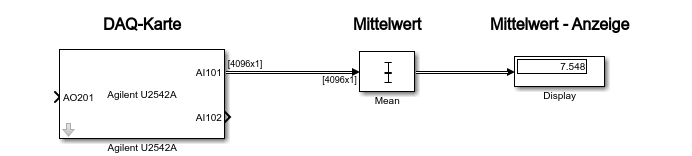
\includegraphics[width=10cm]{assets/kennlinie_aufbau}
		\caption{Simulink Modell zur Bestimmung des Mittelwerts}
	\end{figure}\newline
	Die Ermittlung der Kennlinie wird einmal für den ersten Reflektor und einmal für den zweiten Reflektor durchgeführt.\newline
	\begin{longtable}[h]{|c|c|c|}
			\hline
			\multicolumn{1}{|l|}{\textit{Abstand [mm]}} & \multicolumn{1}{l|}{\textit{U[V] - Reflektor 1}} & \multicolumn{1}{l|}{\textit{U[V] - Reflektor 2}} \\ \hline
			0 & 0.133 & 2.09 \\ \hline
			0.25 & 0.138 & 2.385 \\ \hline
			0.5 & 0.17 & 3.576 \\ \hline
			0.75 & 0.201 & 4.455 \\ \hline
			1 & 0.2085 & 4.592 \\ \hline
			1.25 & 0.2 & 4.258 \\ \hline
			1.5 & 0.1872 & 3.821 \\ \hline
			1.75 & 0.1825 & 3.503 \\ \hline
			2 & 0.1903 & 3.395 \\ \hline
			2.25 & 0.2104 & 3.512 \\ \hline
			2.5 & 0.2406 & 3.835 \\ \hline
			2.75 & 0.2789 & 4.306 \\ \hline
			3 & 0.3203 & 4.899 \\ \hline
			3.25 & 0.3626 & 5.535 \\ \hline
			3.5 & 0.402 & 6.15 \\ \hline
			3.75 & 0.4357 & 6.68 \\ \hline
			4 & 0.4626 & 7.091 \\ \hline
			4.25 & 0.4816 & 7.37 \\ \hline
			4.5 & 0.4933 & 7.523 \\ \hline
			\textbf{4.75} & \textbf{0.4981} & \textbf{7.56} \\ \hline
			5 & 0.4977 & 7.49 \\ \hline
			5.25 & 0.4909 & 7.344 \\ \hline
			5.5 & 0.4796 & 7.136 \\ \hline
			5.75 & 0.4652 & 6.883 \\ \hline
			6 & 0.449 & 6.595 \\ \hline
			6.25 & 0.4308 & 6.288 \\ \hline
			6.5 & 0.411 & 5.971 \\ \hline
			6.75 & 0.3908 & 5.65 \\ \hline
			7 & 0.371 & 5.331 \\ \hline
			7.25 & 0.35 & 5.022 \\ \hline
			7.5 & 0.3302 & 4.716 \\ \hline
			7.75 & 0.311 & 4.424 \\ \hline
			8 & 0.2929 & 4.146 \\ \hline
			8.25 & 0.2757 & 3.888 \\ \hline
			8.5 & 0.2587 & 3.644 \\ \hline
			8.75 & 0.2435 & 3.415 \\ \hline
			9 & 0.229 & 3.198 \\ \hline
			9.25 & 0.215 & 2.999 \\ \hline
			9.5 & 0.2028 & 2.811 \\ \hline
			9.75 & 0.1909 & 2.64 \\ \hline
			10 & 0.1797 & 2.477 \\ \hline
			10.25 & 0.1695 & 2.328 \\ \hline
			10.5 & 0.16 & 2.187 \\ \hline
			10.75 & 0.1511 & 2.057 \\ \hline
			11 & 0.1429 & 1.936 \\ \hline
			11.25 & 0.135 & 1.825 \\ \hline
			11.5 & 0.128 & 1.72 \\ \hline
			\caption{Auswertung der Ausgangsspannung in Abhängigkeit des Abstands für beide Reflektoren}
			\label{tab:my-table}
	\end{longtable}
	Die jeweiligen Maxima der Messungen sind hervorgehoben. Es zeigt sich, dass die Maxima, für beide Reflektoren, bei dem selben Abstand auftreten. Jedoch ist die Spannung bei dem zweiten Reflektor um ein vielfaches höher, was an der höheren Reflektivität und damit der höheren Intensität, des reflektierten Lichtes, liegt.\\ \newline
	Die grafische Darstellung der Kennlinie ergibt eine Parabel. Die Kennlinie hat einen ersten "Gupf" zwischen $0mm$ und $2mm$. Dieser Gupf kommt dadurch zustande, dass reflektiertes Licht am Näherungssensor wieder reflektiert wird und somit die Intensität erhöht.\\ \newline
	\begin{figure}[H]
		\centering
		\begin{tikzpicture}
			\begin{axis}[xlabel={Abstand[mm]}, ylabel={U[V]}]
			\addplot[blue]
			table {assets/reflektor1.csv};
			\addplot[]
			table[header=false,skip first n=1,
			y={create col/linear regression},
			] {assets/reflektor1-regu.csv};  
			\addplot[domain=1.5:5, red]
			{\pgfplotstableregressiona*x + \pgfplotstableregressionb};
			\addplot[]
			table[header=false,skip first n=1,
			y={create col/linear regression},
			] {assets/reflektor1-regd.csv};  
			\addplot[domain=4:10.5, red]
			{\pgfplotstableregressiona*x + \pgfplotstableregressionb};
			\end{axis}
		\end{tikzpicture}
		\caption{Kennlinie - Reflektor 1}
	\end{figure}
	\begin{figure}[H]
		\centering
		\begin{tikzpicture}
			\begin{axis}[xlabel={Abstand[mm]}, ylabel={U[V]}]
			\addplot[blue]
			table {assets/reflektor2.csv};
			\addplot[]
			table[header=false,skip first n=1,
			y={create col/linear regression},
			] {assets/reflektor2-regu.csv};  
			\addplot[domain=1.5:5, red]
			{\pgfplotstableregressiona*x + \pgfplotstableregressionb};
			\addplot[]
			table[header=false,skip first n=1,
			y={create col/linear regression},
			] {assets/reflektor2-regd.csv};  
			\addplot[domain=4:10.5, red]
			{\pgfplotstableregressiona*x + \pgfplotstableregressionb};
			\end{axis}
		\end{tikzpicture}
		\caption{Kennlinie - Reflektor 2}
	\end{figure}
	\noindent
	\underline{\textbf{Analyse der linearen Approximationen}} \\ \newline
	Pro Reflektor wurden zwei Messbereiche definiert, welche annähernd linear verlaufen. Für diese Bereiche wurde die lineare Approximation durchgeführt und die Gerade in der Kennlinie eingezeichnet.\\ \newline
	\begin{figure}[H]
		\centering
		\begin{tikzpicture}
		\begin{axis}[title={Reflektor 1, Messbereich 1}, xlabel={U[V]}, ylabel={Abstand[mm]}]
		\addplot[blue]
		table {assets/reflektor1-abwu.csv};
		\end{axis}
		\end{tikzpicture}
		\caption{Positionsabweichung der Kennlinie von der linearen Approximation - Reflektor 1, Messbereich 1. Maximale Abweichung: 0.2748mm}
	\end{figure}
	\begin{figure}[H]
	\centering
		\begin{tikzpicture}
		\begin{axis}[title={Reflektor 1, Messbereich 2}, xlabel={U[V]}, ylabel={Abstand[mm]}]
		\addplot[blue]
		table {assets/reflektor1-abwd.csv};
		\end{axis}
		\end{tikzpicture}
		\caption{Positionsabweichung der Kennlinie von der linearen Approximation - Reflektor 1, Messbereich 2. Maximale Abweichung: 0.2484mm}
	\end{figure}
	\begin{figure}[H]
		\centering
		\begin{tikzpicture}
		\begin{axis}[title={Reflektor 2, Messbereich 1}, xlabel={U[V]}, ylabel={Abstand[mm]}]
		\addplot[blue]
		table {assets/reflektor2-abwu.csv};
		\end{axis}
		\end{tikzpicture}
		\caption{Positionsabweichung der Kennlinie von der linearen Approximation - Reflektor 2, Messbereich 1. Maximale Abweichung: 0.2928mm}
	\end{figure}
	\begin{figure}[H]
		\centering
		\begin{tikzpicture}
		\begin{axis}[title={Reflektor 2, Messbereich 2}, xlabel={U[V]}, ylabel={Abstand[mm]}]
		\addplot[blue]
		table {assets/reflektor2-abwd.csv};
		\end{axis}
		\end{tikzpicture}
		\caption{Positionsabweichung der Kennlinie von der linearen Approximation - Reflektor 2, Messbereich 2. Maximale Abweichung: 0.2781mm}
	\end{figure}
	\noindent
	In den Abbildung 4 bis 7 ist dargestellt, wie die Kennlinie von der linearen Approximation, im jeweiligen Messbereich, abweicht.\\ \newline
	Die Sensitivität kann mit \[
	E = \frac{\partial U}{\partial d}
	\] berechnet werden. Die Sensitivität kann somit auch als die Steigung der linearen Approximation bezeichnet werden.\\ \newline
	\begin{table}[h]
		\centering
		\begin{tabular}{|c|c|c|}
			\hline
			\textit{} & \textit{Geradengleichung} & $E[\frac{V}{mm}]$ \\ \hline
			\textit{Reflektor 1 Bereich 1} & $0.1212 V/mm * d - 0.0521V$ & $0.1212 V/mm$ \\ \hline
			\textit{Reflektor 1 Bereich 2} & $-0.0646 V/mm * d + 0.8206V$ & $-0.0646 V/mm$ \\ \hline
			\textit{Reflektor 2 Bereich 1} & $1.844 V/mm * d - 0.775V$ & $1.844 V/mm$ \\ \hline
			\textit{Reflektor 2 Bereich 2} & $-1.021 V/mm * d + 12.5952V$ & $-1.021 V/mm$ \\ \hline
		\end{tabular}
		\caption{Sensitivität der Messbereiche}
		\label{tab:my-table}
	\end{table}\newline
	In Tabelle 2 wird ersichtlich, dass die Kennlinie von Reflektor 2 eine deutlich höhere Sensitivität aufweist. Das bedeutet, dass eine Änderung des Abstands eine deutlich höhere Änderung in der Ausgangsspannung, als bei Reflektor 1, verursacht. Das ist von Vorteil, wenn man geringe Abstände messen möchte.\newline
	Möchte man jedoch einen breiteren Messbereich nutzen, wäre der Messbereich 2 des Reflektors 2 zu wählen.\\ \newline
	
	Um die Sensitivität zu erhöhen, muss die Reflektivität des Reflektors erhöht werden.\\ \newline
	Um eine eindeutige Abstandsmessung durchzuführen ist es wichtig genau bestimmen zu können, in welchem Messbereich man sich aktuell befindet (steigend oder fallend).\\ \newline
	\noindent
	\underline{\textbf{Rauschen und Auflösung}} \\ \newline
	Zur Analyse der Rauscheigenschaften, der Schaltung, wird die Leuchtdiode mit einem Gleichspannungs-Signal von $1.5V$ und $0.5V$ versorgt. Als Reflektor wird Reflektor 2 genutzt. Dieser ist so zu positionieren, dass der optische Näherungssensor die maximale Ausgangsspannung liefert (in unserem Fall bei $4.75mm$).\\ \newline
	Mithilfe von Simulink sollen die Standardabweichung und der Spitze-Spitze-Wert gemessen werden. Dazu wurde das Modell gemäß Abbildung 8 erweitert.
	\begin{figure}[h]
		\centering
		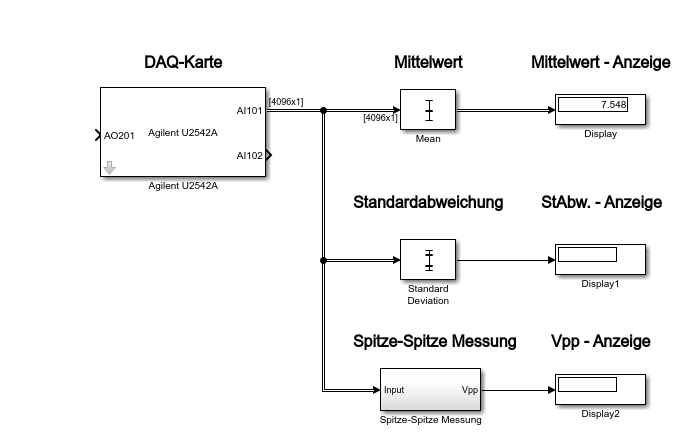
\includegraphics[width=10cm]{assets/rauschen_aufbau}
		\caption{Simulink Modell zur Bestimmung der Standardabweichung und des Spitze-Spitze-Werts des Rauschens}
	\end{figure}
	\newpage
	\noindent
	Die Messung wurde mit einer Abtastfrequenz von $20kHz$, einer daraus resultierenden Abtastzeit von $50\mu s$ und einer Anzahl von $4096 samples$ durchgeführt. Daraus ergibt sich eine Messdauer von \(T_M=\frac{1}{20kHz*4096 samples}=0.2048s\).\\ \newline
	Die Messung wurde bei Tageslicht, mit keiner zusätzlichen Beleuchtung, durchgeführt.\newline
	\begin{table}[h]
		\centering
		\begin{tabular}{|c|c|c|c|}
			\hline
			\textit{$U_e$} & \textit{$U_{mean}[V]$} & \textit{$\sigma[V]$} & \textit{$V_{pp}[V]$} \\ \hline
			$1.5V$ & 7.539 & 0.01327 & 0.1053 \\ \hline
			$0.5V$ & 2.043 & 0.01279 & 0.09308 \\ \hline
		\end{tabular}
		\caption{Bestimmung von Mittelwert, Standardabweichung und Spitze-Spitze-Werts des Rauschens}
		\label{tab:my-table}
	\end{table}\newline
	Bei den Messungen zeigt sich, dass das Rauschen weitestgehend unabhängig von der Eingangsspannung ist. Lediglich der Mittelwert ändert sich, bei einer veränderten Eingangsspannung.\newline
	Da unsere Erwartung war, dass alle Messwerte mit der Eingangsspannung abnehmen, liegt dem vermutlich ein Messfehler zu Grunde.\\ \newline
	Zusätzlich ist festzustellen, dass für gaußförmig verteilte Amplituden der Spitze-Spitze-Wert ungefähr $6\sigma$ entspricht. In unserem Fall entspricht das \(6\sigma = 0,767V bzw. 0,7962\) was kleiner ist als der gemessene Spitze-Spitze-Wert. Der Zusammenhang wird somit nicht erfüllt, was darauf zurückzuführen ist, dass unsere Amplituden nicht gaußförmig sind. Unsere Störeinflüsse entsprechen somit keiner normalen Zufallsverteilung.\\ \newline
	Mögliche Rauschquellen können sein:
	\begin{itemize}
		\item Rauschen in der Spannungsversorgung. Dieser Effekt kann durch passende Filter minimiert werden.
		\item Rauschen durch Umgebungslicht. Kann durch die Abschirmung des Messaufbaus minimiert werden.
		\item Rauschen durch Wärmestrahlung. Da unser optischer Näherungssensor Licht im Infrarot-Bereich aussendet, können thermische Störeinflüsse ebenfalls die Messung beeinflussen. Auch hier kann durch eine geeignete Abschirmung der Effekt minimiert werden.
	\end{itemize}
	Da bei der optischen Abstandsmessung das Rauschen die exakte Position des Messobjekts verfälscht, kann nur ein Bereich angegeben werden, in dem das Objekt sich mit einer hohen Wahrscheinlichkeit befindet.\newline
	Die $6\sigma$-Auflösung ist jener Bereich, in dem der tatsächliche Wert mit einer Wahrscheinlichkeit von $99.7\%$ liegt.\newline
	Die Standardabweichung ist abhängig von der Bandbreite.\\ \newline
	\noindent
	\underline{\textbf{Spektrum der Fremdlichtintensität}} \\ \newline
	Für die folgende Messung wird die Leuchtdiode mit einer Gleichspannung von 0V versorgt. Des weiteren wird das Simulink Modell gemäß Abbildung 9 um einen Spectrum Analyzer erweitert.\\
	Als Störquelle wird eine Glühfadenlampe in einem Abstand von circa $25cm$ über dem optischen Näherungssensor platziert.
	\begin{figure}[h]
		\centering
		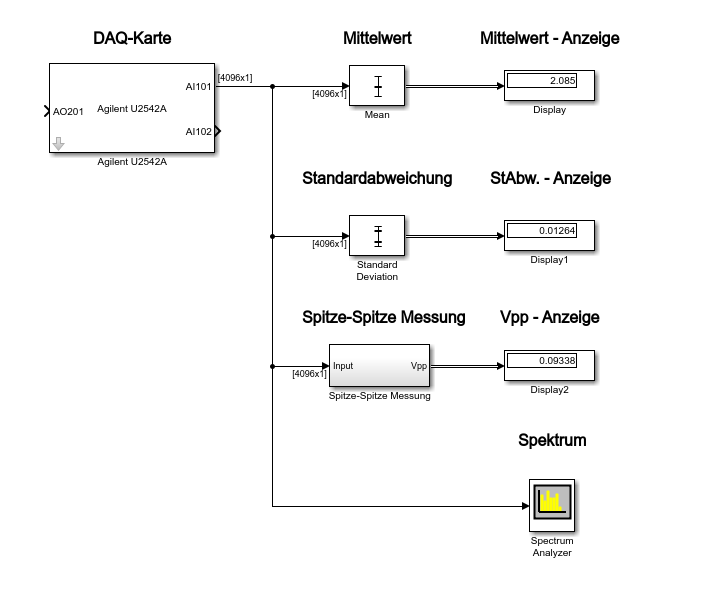
\includegraphics[width=10cm]{assets/rauschen-spektrum}
		\caption{Simulink Modell mit Spectrum Analyzer}
	\end{figure}
	\newpage
	\noindent
	Es wurden mehrere Messungen durchgeführt, bei denen die Störeinflüsse variiert wurden.
	\begin{figure}[H]
		\centering
		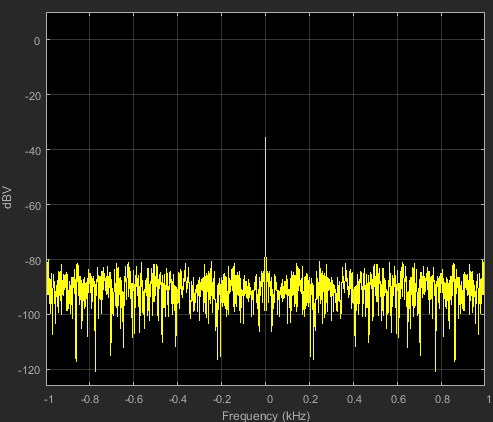
\includegraphics[width=7cm]{assets/lampe-aus}
		\caption{Ausgeschaltete Lampe. Mittelwert: $0.01718V$. Standardabweichung: $0.01232V$. Spitze-Spitze-Wert: $0.08789V$.}
	\end{figure}
	\begin{figure}[H]
		\centering
		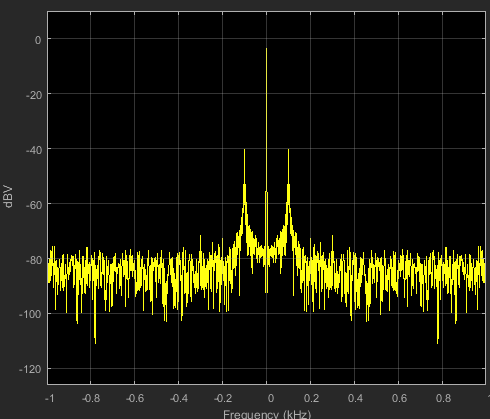
\includegraphics[width=8cm]{assets/lampe-an}
		\caption{Eingeschaltete Lampe. Mittelwert: $0.6646V$. Standardabweichung: $0.02024V$. Spitze-Spitze-Wert: $0.1331V$.}
	\end{figure}
	\begin{figure}[H]
		\centering
		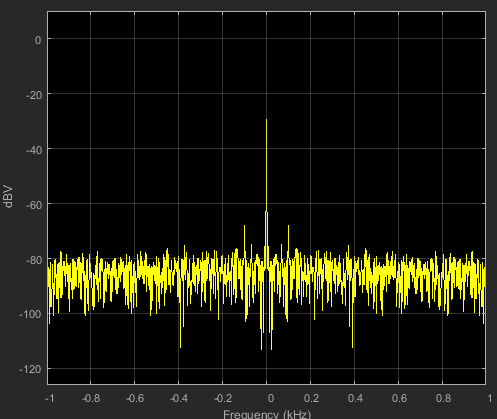
\includegraphics[width=8cm]{assets/raumbel}
		\caption{Ausgeschaltete Lampe mit Raumbeleuchtung. Mittelwert: $0.03695V$. Standardabweichung: $0.01304V$. Spitze-Spitze-Wert: $0.08881V$.}
	\end{figure}
	\begin{figure}[H]
		\centering
		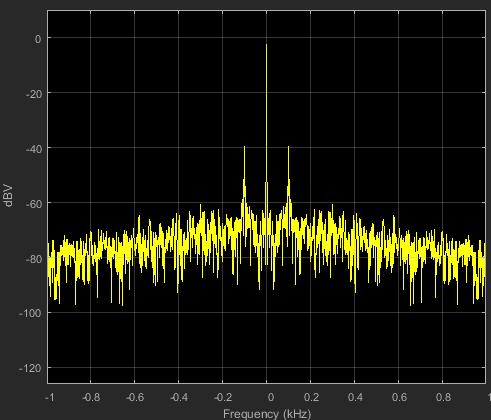
\includegraphics[width=8cm]{assets/lampe-raumbel}
		\caption{Eingeschaltete Lampe mit Raumbeleuchtung. Mittelwert: $0.7425V$. Standardabweichung: $0.02077V$. Spitze-Spitze-Wert: $0.1389V$.}
	\end{figure}
	\noindent
	In Abbildung 13 können markante Frequenzanteile bei $0Hz$, $100Hz$, $200Hz$, $300Hz$, etc. erkannt werden. Diese Anteile kommen großteils von der Glühfadenlampe, welche mit Netzspannung, mit $50Hz$, betrieben wurde.\newline
	Das Licht wird jedoch als Leistungssignal übertragen. Da die Leistung vom Quadrat der Spannung abhängt, ergibt das ein Produkt aus zwei Sinus-Signales mit jeweils $50Hz$. Im Frequenzbereich ergibt das Anteile bei $0Hz$ und $100Hz$. Da die Kennlinie der Leuchtdiode nicht linear ist, erzeugt die Taylor-Entwicklung die weiteren Ausschläge bei $200Hz$, $300Hz$, $400Hz$, etc.\newline
	Zusätzlich fließen die $0Hz$ der Gleichspannungs Eingangsspannung in den markanten Frequenzanteil bei $0Hz$ mit ein.\\ \newline
	In Abbildung 10 zeigt sich, dass sie oben genannten markanten Frequenzanteile verschwinden, da die Glühfadenlampe nicht mehr als Störquelle aktiv ist.\newline
	\newpage
	\subsection{Phasenselektiver Synchrongleichrichter}
	\underline{\textbf{Aufgabenstellung}} \\ \newline
	\noindent
	Ziel dieser Aufgabe ist es die Funktionsweise eines Phasenselektiver Synchrongleichrichters kennen zu lernen. Zusätzlich sollen die Vor- und Nachteile erarbeitet werden.\\ \newline
	\underline{\textbf{Allgemeine Funktionsweise}} \\ \newline
	\noindent
	Der Phasenselektiver Synchrongleichrichter, auch PSSG genannt, dient zum Messen der Amplitude einer bestimmten Frequenz, aus einem Mischsignal.\newline
	\begin{figure}[h]
		\centering
		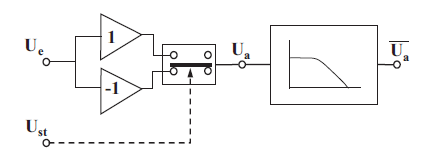
\includegraphics[width=10cm]{assets/pssg}
		\caption{Aufbau eines PSSG mit einem Tiefpassfilter zur Mittelwertbildung.}
	\end{figure}\newline
	Der PSSG wird mit einem Steuersignal versorgt, welches in der selben Frequenz, wie das Eingangssignal, schwingt. Hierfür wird ein Rechtecksignal genutzt.\newline
	Im PSSG wird das Eingangssignal, durch das Steuersignal, abwechselnd invertiert und nicht-invertiert. Dadurch wird der Anteil bei $f_{st}$ gleichgerichtet.\newline
	Da es zu Messfehlern kommt, wenn die Frequenz des Steuersignals nicht gleich der Frequenz des Eingangssignals ist, muss sowohl die Frequenz, als auch der Phasenwinkel des Eingangssignals bei der Messung bekannt sein.
	\begin{figure}[H]
		\centering
		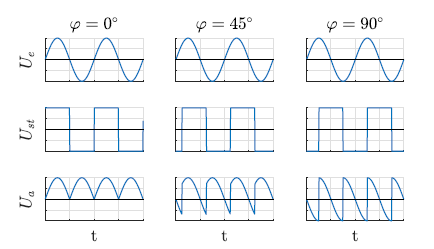
\includegraphics[width=10cm]{assets/signale-pssg}
		\caption{Signalverläufe des PSSGs in Abhängigkeit von der Phasenverschiebung.}
	\end{figure}
	\noindent
	\underline{\textbf{Messaufbau}} \\ \newline
	\noindent
	Der Phasenselektiver Synchrongleichrichter wird in Simulink aufgebaut.\newline
	Um keine Abweichung bei der Frequenz oder dem Phasenwinkel zwischen dem Eingangssignal und dem Steuersignal zu erhalten, werden beide Signale vom selben Kanal am Frequenzgenerator versorgt. Das Eingangssignal ist somit gleich dem Steuersignal.\\ \newline
	Am Frequenzgenerator wird ein Sinus-Signal mit $0.4V_{pp}$, einem Offset von $1.3V$ und einer Frequenz von $60Hz$ eingestellt.\newline
	\begin{figure}[h]
		\centering
		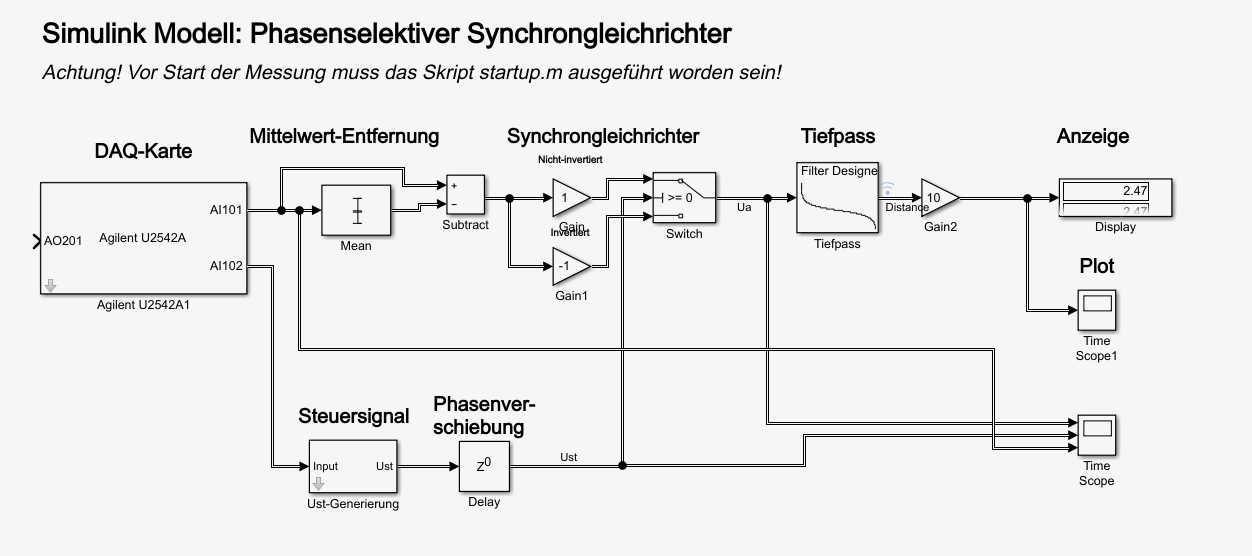
\includegraphics[width=10cm]{assets/pssg-modell}
		\caption{Simulink Modell des Phasenselektiver Synchrongleichrichters.}
	\end{figure}\newline
	Da der Mittelwert des Signals im realen Fall, aufgrund der endlichen Abtastschritte, nicht ausgelöscht wird, muss er am Eingangs des PSSG vom Signal abgezogen werden.\\ \newline
	Als Tiefpassfilter wird ein Butterworth-Tiefpass zehnter Ordnung, mit einer Grenzfrequenz von $3Hz$ gewählt.\\ \newline
	\textbf{Leider gab es während der Messung Probleme mit der DAQ-Karte, an unserem Laborplatz. Später stellte sich heraus, das die DAQ-Karte eigentlich von einem anderen Messplatz stammt, wo sie als defekt deklariert wurde. Alle weiteren Messungen wurden daher zusammen mit einem anderen Dreierteam der Gruppe 2 durchgeführt.}\\ \newline
	\underline{\textbf{Darstellung bei verschiedenen Phasenlagen}} \\ \newline
	\noindent
	Um eine Phasenverschiebung von $0^{\circ}$ zu erreichen, wurden im Delay-Block des Simulink Modells 0 Samples konfiguriert.\newline
	\begin{figure}[h]
		\centering
		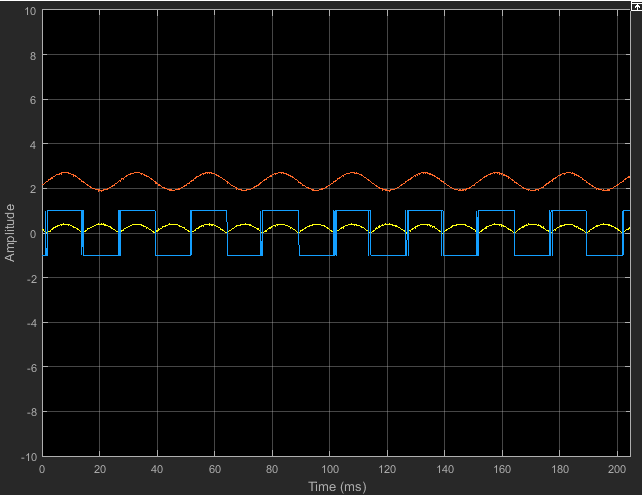
\includegraphics[width=10cm]{assets/pssg-phase0}
		\caption{Signale des PSSG bei $0^{\circ}$ Phasenverschiebung}
	\end{figure}\newline
	Das Ausgangssignal (gelb) zeigt, dass das Eingangssignal (rot) korrekt gleichgerichtet wurde.\\ \newline
	Um eine Phasenverschiebung von $45^{\circ}$ zu erreichen, muss die Anzahl der Samples, zum Verschieben, errechnet werden.\newline
	Da wir mit einer Abtastfrequenz von $20kHz$ arbeiten und das Eingangssignal $60Hz$ beträgt, ergibt sich die Anzahl der Samples zu \[
		\frac{45^{\circ}}{360^{\circ}}=\frac{n_{45^{\circ}}}{n_{360^{\circ}}}=\frac{n_{45^{\circ}}}{\frac{f_S}{f_M}}
	\]
	\[
		n_{45^{\circ}}=\frac{f_S}{f_M}\frac{n_{45^{\circ}}}{n_{360^{\circ}}}=42 Samples
	\]
	\begin{figure}[H]
		\centering
		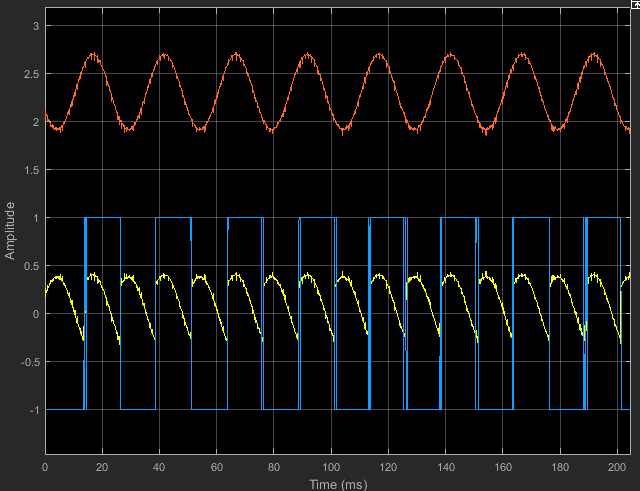
\includegraphics[width=10cm]{assets/pssg-phase45}
		\caption{Signale des PSSG bei $45^{\circ}$ Phasenverschiebung}
	\end{figure}
	\noindent
	Um eine Phasenverschiebung von $90^{\circ}$ zu erreichen, muss der Delay-Block auf $84 Samples$ konfiguriert werden.\newline Die Berechnung erfolgt analog zur Berechnung für eine Phasenverschiebung von $45^{\circ}$.
	\begin{figure}[H]
		\centering
		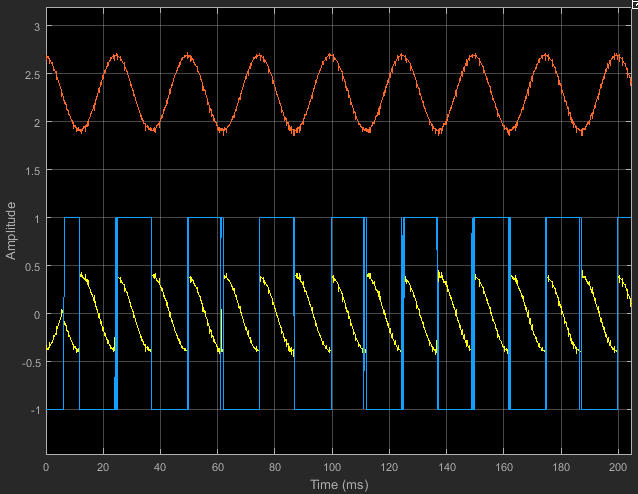
\includegraphics[width=10cm]{assets/pssg-phase90}
		\caption{Signale des PSSG bei $90^{\circ}$ Phasenverschiebung}
	\end{figure}
	\noindent
	Wie in Abbildung 19 dargestellt, ist das Ausgangssignal, bei einer Phasenverschiebung von $90^{\circ}$, mittelwertfrei.\\ \newline
	\underline{\textbf{Messungen mit dem PSSG}} \\ \newline
	\noindent
	Für diese Aufgabe wurde der Reflektor so positioniert, dass das Ausgangssignal eine Amplitude von circa $0.5V$ hat. Die Glühfadenlampe ist im ersten Schritt noch ausgeschaltet. \newline
	Als nächstes wird die Glühfadenlampe in einem Abstand von circa $15cm$ platziert.\\ \newline
	Am Frequenzgenerator werden $100.5Hz$ eingestellt um die Störung im Ausgangssignal der Lampe, bei $100Hz$, sichtbar zu machen.\newline
	Bei exakt $100Hz$ wäre die Störung nur als Gleichanteil sichtbar.
	\begin{figure}[H]
		\centering
		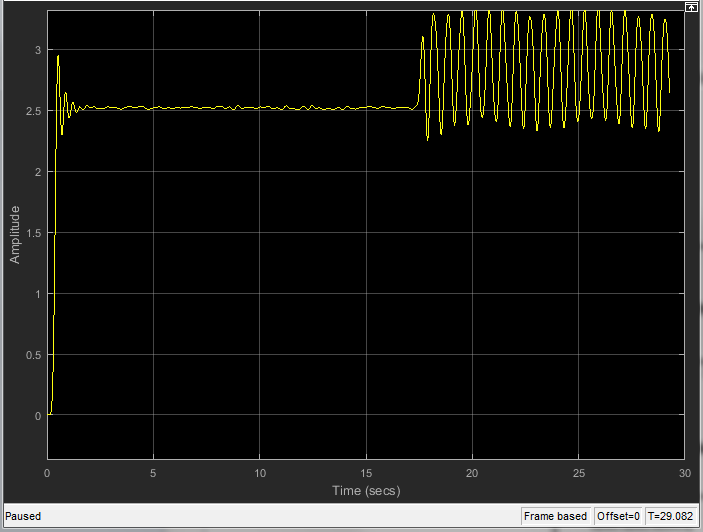
\includegraphics[width=10cm]{assets/pssg-100_5Hz}
		\caption{Ausgangssignal mit Einschaltvorgang, bei $100.5Hz$. Links ohne Störung, rechts mit $100Hz$ Störung}
	\end{figure}
	\noindent
	Die Störung bei $100Hz$ zeigt sich in Abbildung 20 rechts als niederfrequente Schwingung, da die Faltung des $100.5Hz$ Rechtecks (unser Steuersignal) eine $~0.5Hz$ Schwingung erzeugt, die der Tiefpass durchlässt.\\ \newline
	Die selbe Störung zeigt sich ebenfalls bei $20Hz$ (siehe Abbildung 21) und $33.4Hz$ (siehe Abbildung 22), da diese die 3. und 5. Oberwelle des Steuersignals sind.
	\begin{figure}[H]
		\centering
		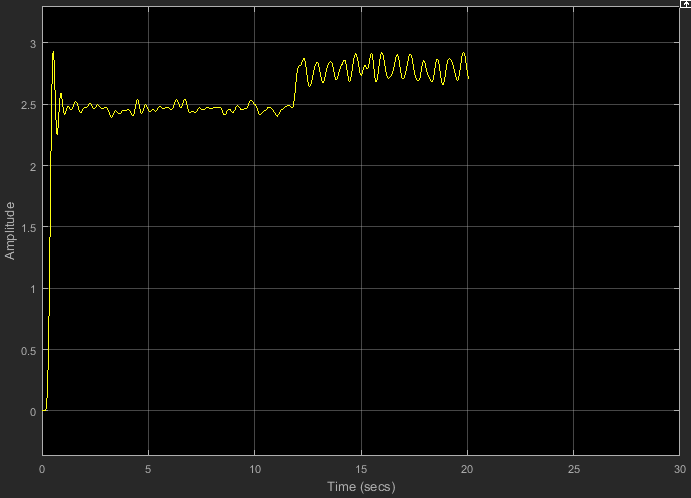
\includegraphics[width=10cm]{assets/pssg-20Hz}
		\caption{Ausgangssignal mit Einschaltvorgang, bei $20Hz$. Links ohne Störung, rechts mit Störung}
	\end{figure}
	\begin{figure}[H]
		\centering
		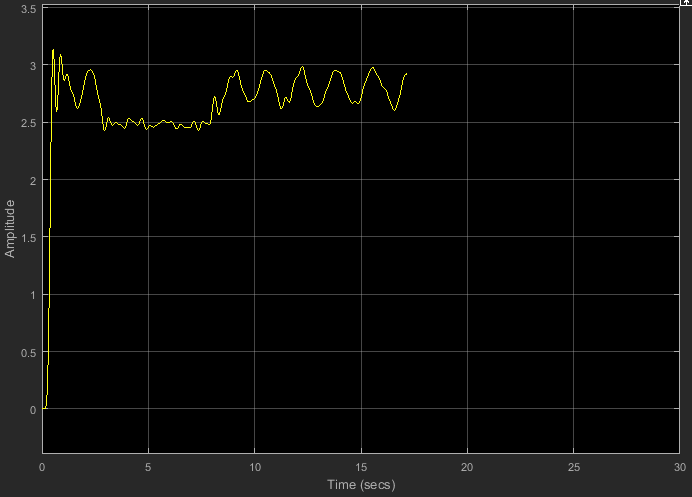
\includegraphics[width=10cm]{assets/pssg-33_4Hz}
		\caption{Ausgangssignal mit Einschaltvorgang, bei $33.4Hz$. Links ohne Störung, rechts mit Störung}
	\end{figure}
	\noindent
	Bei $75.1Hz$ tritt zum Beispiel keine Störung auf, da die Frequenz keine Oberwelle des Steuersignals ist.\newline
	\begin{figure}[H]
		\centering
		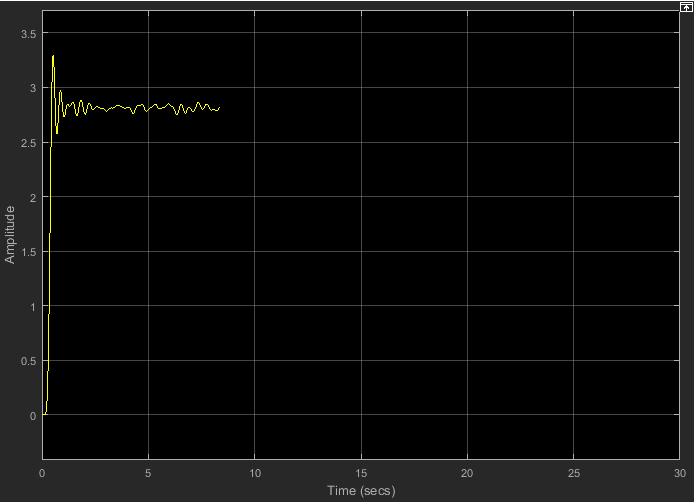
\includegraphics[width=10cm]{assets/pssg-75_1Hz}
		\caption{Ausgangssignal mit Einschaltvorgang, bei $75.1Hz$. Keine Störung}
	\end{figure}
	\noindent
	Störungen treten auf, sobald ungeradzahlige Harmonische, aus der Multiplikation des Sinus bei $f_{st}$ mit dem Steuersignal, auf eine Frequenz fallen, wo ein Störsignal liegt.\\ \newline
	\begin{longtable}[c]{|c|c|c|}
		\hline
		\textit{$Frequenz[Hz]$} & \textit{Störung erwartet?} & \textit{Störung gemessen?} \\ \hline
		\endfirsthead
		%
		\endhead
		%
		20.1 & Ja & Ja \\ \hline
		33.4 & Ja & Ja \\ \hline
		50.1 & Nein & Nein \\ \hline
		75.1 & Nein & Nein \\ \hline
		100.1 & Ja & Ja \\ \hline
		125.1 & Nein & Nein \\ \hline
		150.1 & Nein & Nein \\ \hline
		175.1 & Nein & Nein \\ \hline
		200.1 & Nein & Nein \\ \hline
		\caption{Messergebnisse bei unterschiedlichen Messfrequenzen mit dem PSSG}
		\label{tab:my-table}\\
	\end{longtable}
	\newpage
	\subsection{Phasenunabhängiger Synchrondemodulator}
	\underline{\textbf{Aufgabenstellung}} \\ \newline
	\noindent
	Ziel dieser Aufgabe ist es die Funktionsweise eines Phasenunabhängiger Synchrondemodulator kennen zu lernen. Zusätzlich sollen die Vor- und Nachteile erarbeitet werden.\\ \newline
	\underline{\textbf{Allgemeine Funktionsweise}} \\ \newline
	\noindent
	Der Phasenunabhängiger Synchrondemodulator, auch PUSD genannt, wird, wie der PSSG, verwendet um Amplituden bei einer bestimmten Frequenz zu messen.\newline
	Im Gegensatz zum PSSG bietet der PUSD mehrere Vorteile.
	\begin{itemize}
		\item Die Phasenlage des Eingangssignals muss nicht bekannt sein.
		\item Die Frequenz des Eingangssignals muss nur bis auf den Durchlassbereich der Tiefpassfilter bekannt sein.
		\item Es kommt zu keinen Störung bei Vielfachen des Steuersignals.
	\end{itemize}
	Der Aufbau eines Phasenunabhängige Synchrondemodulators ist in Abbildung 24 dargestellt.\newline
	\begin{figure}[H]
		\centering
		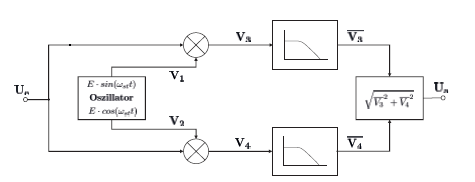
\includegraphics[width=10cm]{assets/pusd}
		\caption{Aufbau eines PUSD}
	\end{figure}
	\noindent
	\underline{\textbf{Messaufbau}} \\ \newline
	\noindent
	Der Aufbau des PUSD erfolgt wieder in Simulink. Das Modell wird dazu gemäß Abbildung 25 angepasst.
	\begin{figure}[H]
		\centering
		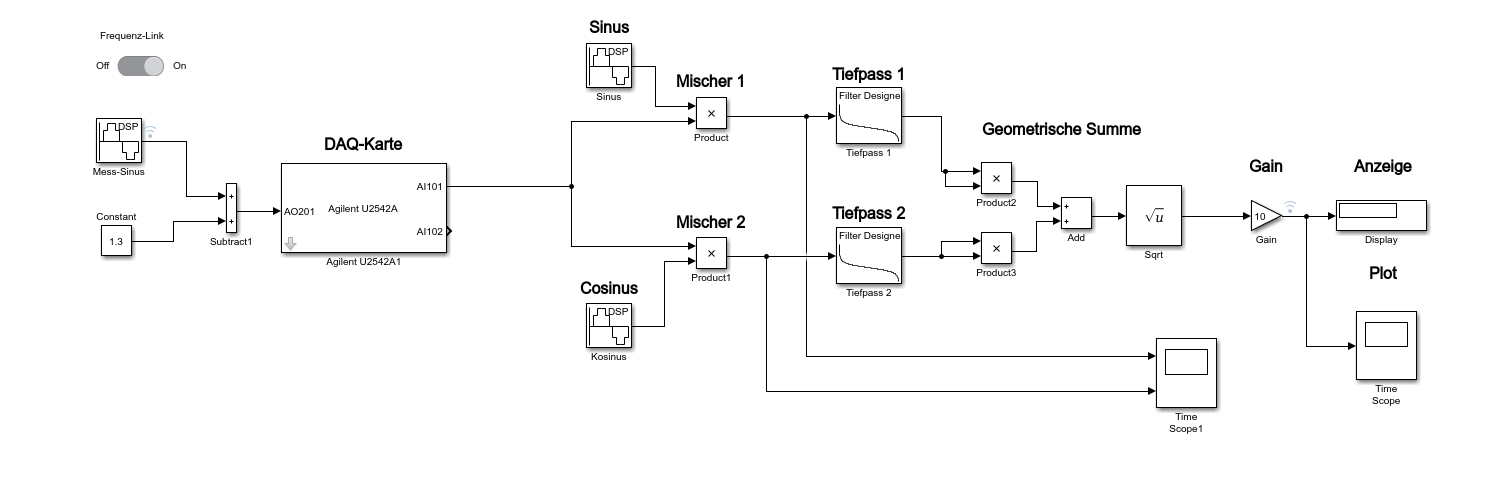
\includegraphics[width=15cm]{assets/pusd-modell}
		\caption{Simulink Modell eines PUSD}
	\end{figure}
	\noindent
	Im Gegensatz zum Messaufbau des PSSG wird statt dem externen Frequenzgenerator die DAQ-Karte genutzt.\newline
	Über den Mess-Sinus Block wird ein Sinus-Signal mit einer Amplitude von $0.2V$ und einem Offset von $1.3V$ eingestellt.\newline
	Die Frequenz kann frei gewählt werden. Bei dem PUSD ist das einzige Kriterium für die Wahl der Frequenz, dass in der Nähe von $f_{st}$ keine Störungen auftreten dürfen.\newline
	Als Tiefpässe werden zwei Butterworth-Tiefpässe zehnter Ordnung, mit einer Grenzfrequenz von $5Hz$ konfiguriert.\\ \newline
	\underline{\textbf{Messungen mit dem PUSD}} \\ \newline
	\noindent
	Wie bereits bei den Messungen mit dem PSSG wird auch für diese Aufgabe der Reflektor 2 so platziert, dass das Ausgangssignal eine Amplitude von circa $0.5V$ hat.\newline
	Die Glühfadenlampe wird wieder in einem Abstand von ungefähr $20cm$ positioniert und bleibt vorerst noch ausgeschaltet.\newline
	Um die $100Hz$-Störung der Lampe sichtbar zu machen, wird in Simulink eine Frequenz von $102Hz$ eingestellt.\newline
	Aus der Messfrequenz von $102Hz$ und der Bandbreite der Tiefpässe von $5Hz$ resultiert eine Empfindlichkeit der Schaltung auf $97Hz$ bis $107Hz$.\\ \newline
	Wieder wurden Messungen bei $21Hz$, $33.4Hz$, $102Hz$ und $110Hz$ durchgeführt.\newline
	\begin{figure}[H]
		\centering
		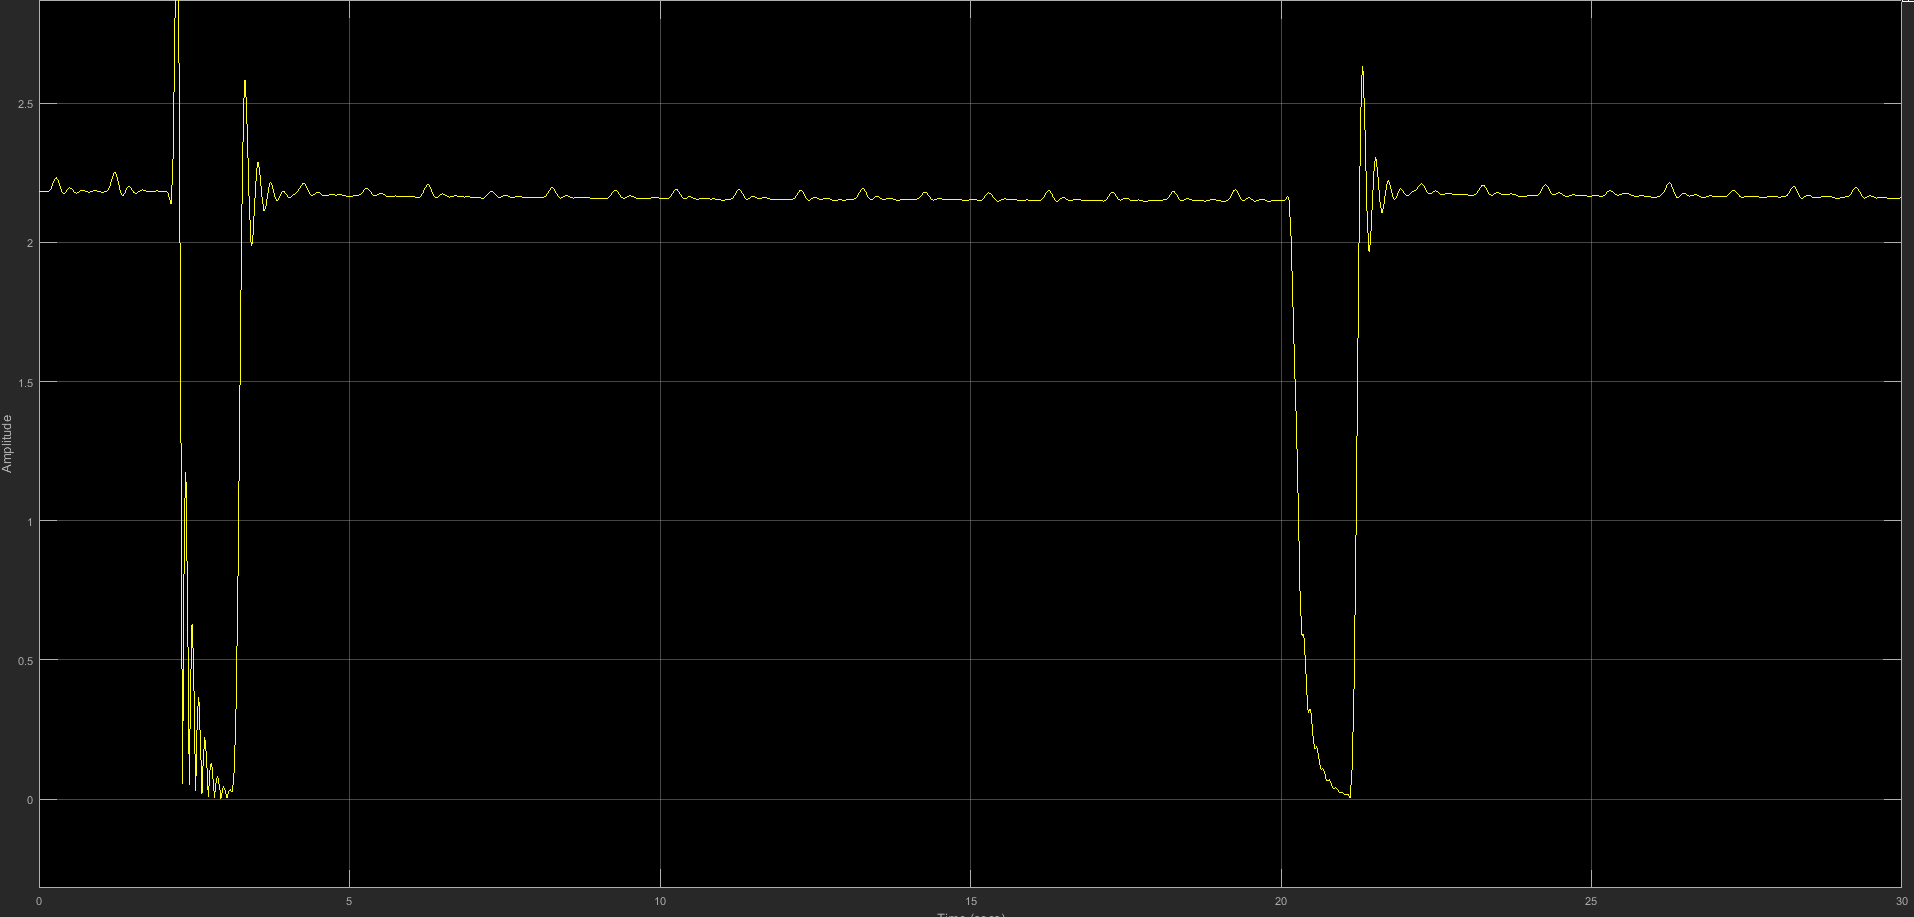
\includegraphics[width=10cm]{assets/pusd_21Hz_34_Hz}
		\caption{Messung bei angeschalteter Lampe. Links mit $21Hz$, rechts mit $34Hz$ Ausgangsspannung. In beiden Fällen tritt keine Störung auf.}
	\end{figure}
	\begin{figure}[H]
		\centering
		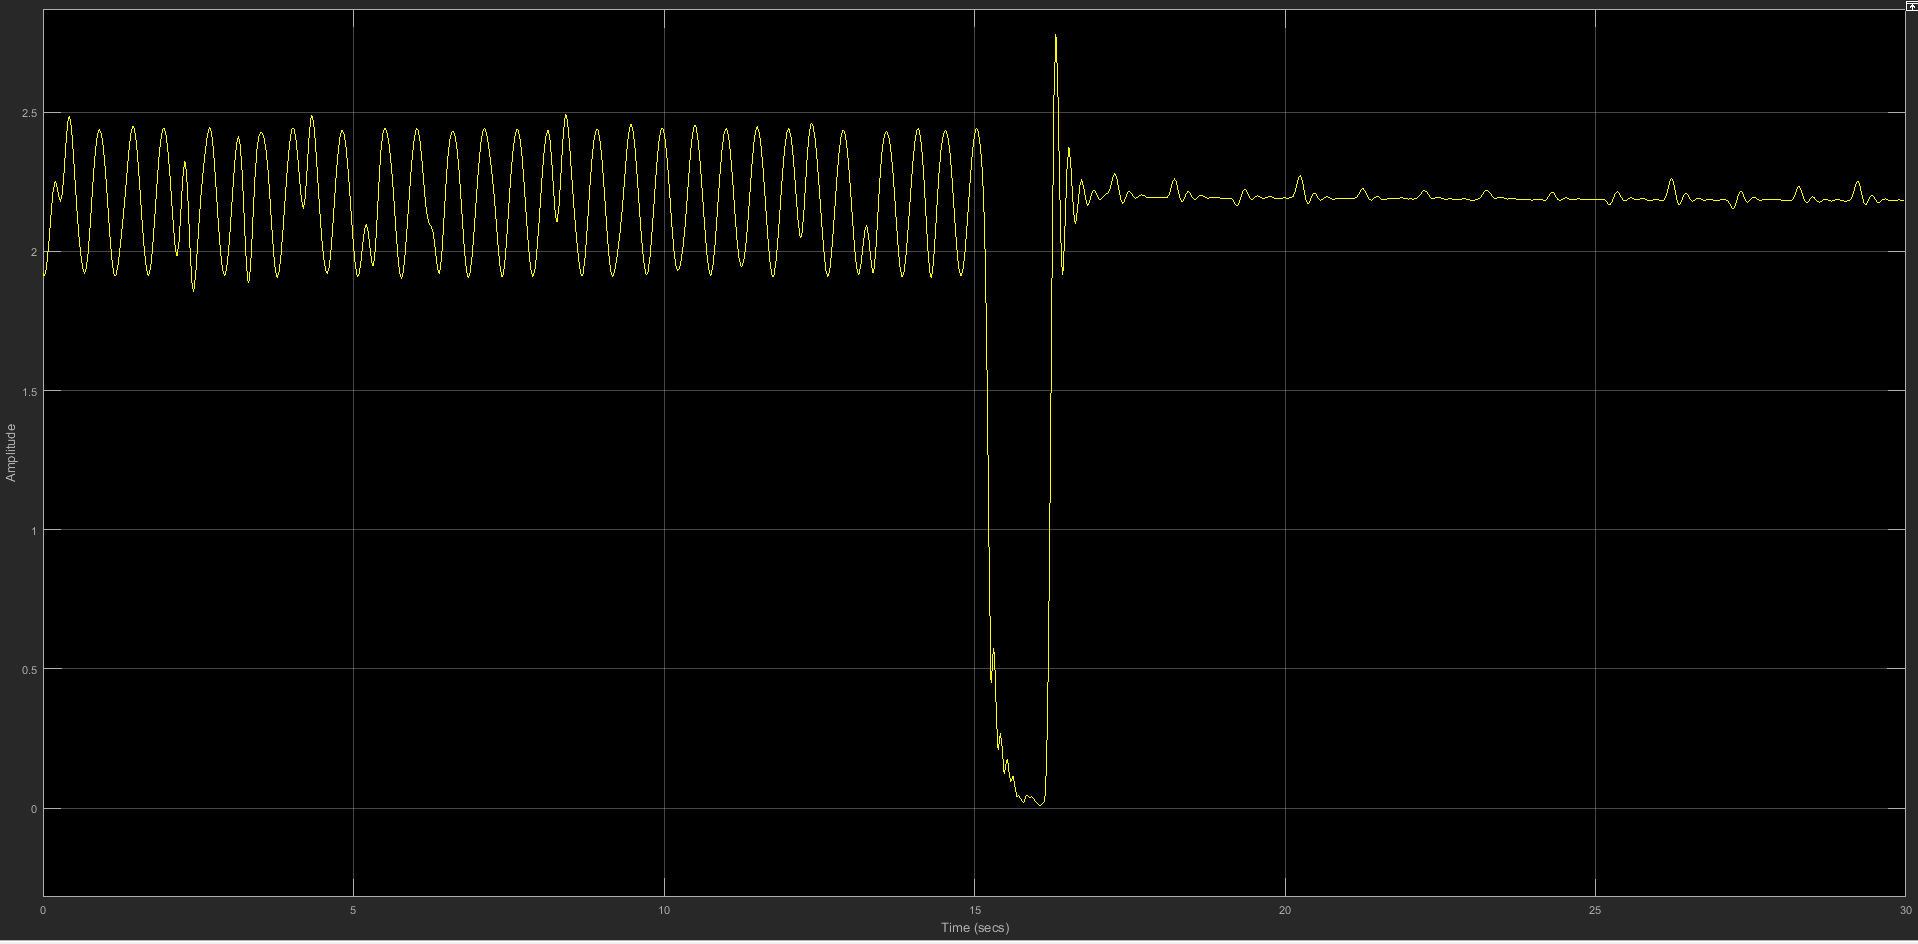
\includegraphics[width=10cm]{assets/pusd_102Hz_110_Hz}
		\caption{Messung bei angeschalteter Lampe. Links mit $102Hz$, rechts mit $110Hz$ Ausgangsspannung. Bei $102Hz$ ist, wie erwartet, eine Störung sichtbar.}
	\end{figure}
	\noindent
	Eine Störung tritt lediglich bei $102Hz$ auf, da sich die Frequenz im Messbereich befindet.\newline
	Weitere Störungen bei ungeradzahligen Harmonischen des Steuersignals, wie beim PSSG, gibt es beim PUSD nicht.\newline
	% Please add the following required packages to your document preamble:
	% \usepackage{longtable}
	% Note: It may be necessary to compile the document several times to get a multi-page table to line up properly
	\newpage
	\begin{longtable}[c]{|c|c|c|}
		\hline
		\textit{$Frequenz [Hz]$} & \textit{Störung erwartet?} & \textit{Störung gemessen?} \\ \hline
		\endfirsthead
		%
		\endhead
		%
		20.1 & Nein & Nein \\ \hline
		33.4 & Nein & Nein \\ \hline
		50.1 & Nein & Nein \\ \hline
		75.1 & Nein & Nein \\ \hline
		100.1 & Ja & Ja \\ \hline
		125.1 & Nein & Nein \\ \hline
		150.1 & Nein & Nein \\ \hline
		175.1 & Nein & Nein \\ \hline
		200.1 & Nein & Nein \\ \hline
		\caption{Messergebnisse bei unterschiedlichen Messfrequenzen mit dem PUSD}
		\label{tab:my-table}\\
	\end{longtable}
	\noindent
	Als Unterschied zur Messung mit dem PSSG ist somit zu nennen, dass Störungen, bei ungeradzahligen Harmonischen des Steuersignals beim PUSD die Messung nicht beeinflussen.\newline
	\newpage
	\section{Verwendete Geräte}
	\begin{itemize}
		\item Agilent U2542A - DAQ-Karte
		\item Honeywell HOA1404-002 - Optischer Näherungssensor
		\item Rigol DP832 - Spannungsversorgung
		\item Agilent DSO-X 2002A - Digitales Oszilloskop
	\end{itemize}
	\newpage
	\listoffigures
	\newpage
	\newpage
	\listoftables
	\newpage
\end{document}